%\documentclass[english]{article}
\documentclass[letterpaper,12pt]{article}
\usepackage[T1]{fontenc} 
\usepackage[utf8]{inputenc}
%\usepackage{babel}
%\usepackage[margin=1.0in]{geometry}
\usepackage[top=0.9in,bottom=0.9in,right=0.9in,left=0.9in ]{geometry}
\usepackage{mathtools,amssymb,amsmath,amsfonts,amsthm,bbm}
\usepackage{booktabs,multirow,multicol}
\usepackage{physics,tensor,slashed}
\usepackage{pgfplots,pdfpages,graphicx}
\usepackage{float}
\usepackage{upgreek}
\usepackage{wrapfig}
\usepackage{enumitem}
\usepackage{xcolor}

\usepackage{caption, setspace}
\captionsetup[table]{font={stretch=1.1}}     %% change 1.2 as you like
\captionsetup[figure]{font={stretch=1.1}}   

\usepackage{fancyhdr}
\pagestyle{fancy}
\fancyhf{}
\renewcommand{\headrulewidth}{0pt}
\fancyhead[R]{\thepage}

\usepackage{titlesec}
\titleformat{\section}{\bfseries\centering\MakeUppercase\large}{}{0pt}{\MakeUppercase}


\setlength{\columnsep}{0.6cm}
\usepackage{CJKutf8}
\makeatletter
\makeatother
\renewcommand{\baselinestretch}{1.5}
%\renewcommand{\thesection}{\textbf{\MakeUppercase{\large{Problem \arabic{section}}}}}
%%% some commands --------------------------------------
\newcommand{\parfrac}[2]{\frac{\partial #1}{\partial #2} }
\newcommand{\sparfrac}[2]{\frac{\partial^2 #1}{\partial #2 ^2} }
\newcommand{\derfrac}[2]{\frac{d #1}{d #2} }
\newcommand{\sderfrac}[2]{\frac{d^2 #1}{d #2 ^2} }
\newcommand{\bracket}[1]{\left(#1\right)}
\newcommand{\cD}{\mathcal{D}}
\newcommand{\cL}{\mathcal{L}}
%\newcommand{\norm}[1]{\left\lVert#1\right\rVert}

\numberwithin{equation}{section}
\begin{document}
%\author{Cunwei Fan}
%\title{\textbf{{PHYS 575 Problem Set 1}}}
%\date{cfan11}
%\maketitle
\clearpage
\thispagestyle{empty}
\begin{center}
    %\vspace*{\stretch{0.5}}
    \Large{\textbf{Project on Limit Order Book of a Specific Stock}}\\
    \large{Cunwei Fan \begin{CJK}{UTF8}{gkai}{(范存炜)}\end{CJK}}
\end{center}


\tableofcontents

%\noindent \textbf{\MakeUppercase{\large{Problem 1} }}
\newpage 
\section{Introduction}

The Limit Order Book (LOB) is a financial tool for people to trade and try to profit or control their own risks. In the nice review \cite{gould2013limit}, the LOB is treated through a mathematical approach. An LOB is an ordered collection of three vectors $(t, p, w)$. Here, $t$ is the time where the order is made and $p$ is the price the order want to transact on and $w$ is quantity concerned in the order. If $w$ is less than $0$, this order is a buying order and if $w >0$, the order is a selling order. The philosophy of the order book is that once there is an order made with matching prices, the order will be conducted and if all quantities are matched then the order is gone. For example, when a trader throw in an order of buying $3$ units on price $5\pi $ where $\pi$ is the price unit, then if there are people selling it with price less or equal to $5\pi$ then the two orders matched and both of them will be cleared from the LOB collection. This rewards people who acts later since if the selling trader wants to trade on price $4\pi$ but a buying order with $5\pi$ comes, then the selling trader could only get $4\pi$ and the buying trader only gets what he or she wants at price of $4\pi$ which is lower than what he or she predicts. Based on this mechanism, there are two kinds of orders, one is \textit{market order} and the other is the \textit{limit order}. The immediate matched order is the market order and the order that is not matched is the limit order. The LOB by its name only stores the limit orders. As a result of the limit orders, the least price of all selling orders must always larger than the buying price of the buying orders for all orders in the limit book. The two prices are denoted by $a(t)$ and $b(t)$ for lowest asking price and the highest bidding price in the LOB. There are a lot of minor rules in different LOB trading system that will affect the traders' behaviour and the nice review and discussion is done in \cite{gould2013limit}. 

In this project, we will focus on an order book of an unknown stock in the market. We will focus on the laws and statistical behaviours of the order flows (the arrival of bidding and asking limit orders), which is a representation of the market trading strategy. We will only focus on small time scale behaviour and our data is only on May 24th, May 25th, May 26, May 31st and June 1st in 2017. The sampling frequency in the order book is around 2 minutes. In this project, we want to dig out the statistical trend of the behaviour of asking and bidding arrivals and try to predict the quantity of asking and bidding orders on the next time point.

In order to solve the problem, we first find out the autocorrelation on the quantity of the ask and bidding orders indicates that the time series of the orders is a long memory process \cite{bhansali2003prediction}. Although, there is some standard approach of studying the long memory approach using fractional Laplacian and ARIMA models, we still want to call to recent development in long signal processing, the WaveNet structure \cite{DBLP:journals/corr/OordDZSVGKSK16}. We would use the net predict both the probability of arrivals of orders as well as the quantity of it using purely the information from the arrival sequence itself. Finally, we would let the predictions be features on the data set and combing these quantities with others to make predictions. 

Simultaneously, we would use the original dataset, after proper scaling, to try to do predictions by just using the features at the instant as well as the features from the previous time step. This prediction only predicts the arrival of orders with information for the instant without considering the old history. In section 3, we will see how we could construct features based on the behaviour observed in the data. Then, we would use Lasso penalty to select useful features and try to do PCA over the whole dataset to make the number of features around the number of features selected by Lasso regression. 
Finally, we will combine the PCA features and the deep net results to do hyper parameter tuning for each model. At last, we would stacking the statistical models together to do the prediction. 

In the last, we will summarize our results and provide some thoughts on how to make our model to behave better for future use. 



\section{Deep Net Sturcture and Loss Design}

In this section, we will first discover the series of the order arrival sequence is a long memory process and second we will describe the WaveNet, a deep CNN model we used for this problem. 

\subsection{Long Memory of Order Arrivals}

We will first detect the long memory process by plotting the autocorrelation (ACF) plot of the data. 
For autocorrlation plot, we are plotting correlation of the sequence with itself in the previous time points. In fact, we define the autocorrelation as 

\begin{equation}
\gamma(s,t) = \frac{\text{Cov}(X_t, X_s)}{\text{Var}(X_t),\text{Var}(X_s) } .
\end{equation}

For stationary process, the autocorrelation only depends on the the time difference. Thus, we would estimate the autocorrelation for fixed value of $h \equiv |s - t|$ since we would have a lot of samples for the fixed time difference. From the below plot, we see the ACF is quite stationary and there is no fictious osicllating behaviour and thus the process is quite stationary. 

The definition of long memory is $$\sum_{h=0}^\infty \gamma(h)  \text{\quad  diverges a.s.}$$
and this is equivalent to if $\gamma(h) \rightarrow h^{- \alpha} $ if $\alpha > 1$. 

Form the below plot, we see both ask and bid arrivals have decay exponents around $-0.2$ for correlations length $h< e^6 \approx 400$. Thus, the autocorrelation could be assumed to be zero since they are round $e^{-4.5} \approx 0.01$. Also, as the lag increases, the autocorrelation plot is more variant and the data should not be trusted. The coefficient we fitted here are $-0.278$ for ask arrival and $-0.21$ for bid arrivals. This would mean that the processes have long memory and we should deal with it explicitly.

\begin{figure}
    \centering
    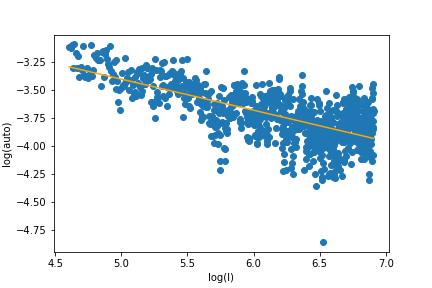
\includegraphics[scale = 0.5]{figs/ACF_ask.png}
    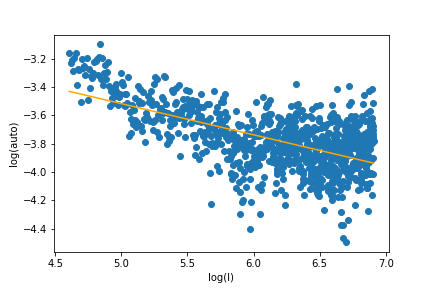
\includegraphics[scale = 0.5]{figs/ACF_bid.png}
    \caption{\small ACF plot for ask and bid arrivals. LEFT: the plot of ACF for ask arrival in log scale and the linear regression on the log scale. RIGHT: the plot of the ACF for bid arrivals in log scale and the linear regression on the log scale. }
    \label{sec2:fig:acf_plot}
\end{figure}

\subsection{Causality CNN: WaveNet}
Because long memory process is complicated and simple ARIMA model with small values for AR and MA would not be enough, we would need to design new models for it.  Although, there exist classical methods such as ARFIMA which uses non local operators like fractional Laplacian to generate long memory process using short memory ARIMA model, we would resort to the deep neural net for help. 

In this project, since we try to extract long memory auto-dependence of the sequence itself, we would not need a very complicated model. Since as shown in \cite{zhao2020rnn}, the LSTM and RNN have memory exponentially decay in the history. Thus, we resort to the WaveNet structure, a CNN structure designed by DeepMind \cite{DBLP:journals/corr/OordDZSVGKSK16}. They focused on how to reduce the number of layers to make the receptive field large enough to take almost all of the data in the sequence. They also put a lot of efforts on causality preserving and they solve it by shifting. In this problem, however, we assume every prediction uses a fixed number of past points to predict and we call this number the \textit{window size}. Then the causality is preserved. Then, we applied the dilation CNN where the receptive field increases exponentially with the number of layers. Then, we uses $7$ layers of dilation convolution and filter size of $3$ which means the output sequence has dependence of $2^8 = 256$ points which is half our window size. The layers of the convolution are connected by residuals which allows better behaving of the gradient. 
Then, in the last we use two layers of fully connected layer which takes all information in the last. The output is two numbers. The first number indicates the probability of arrival and the second number indicates the number of arrivals. 


\begin{figure}
    \centering
    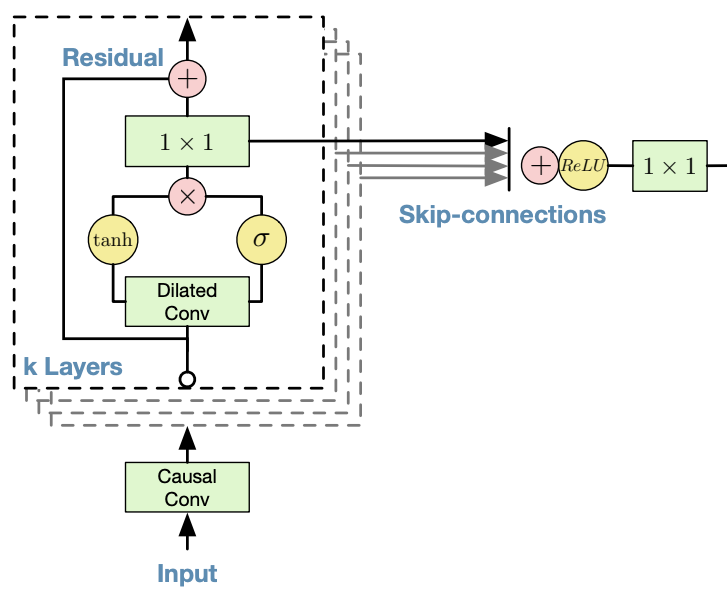
\includegraphics[scale = 0.4]{figs/wavent.png}
    \caption{\small The residual structure of the WaveNet where each layer has exponentially increasing dilation parameter to increase the number of receptive fields}
    \label{fig:my_label}
\end{figure}


In order to train a good model, we should design a good loss function. For ask or bid arrivals, we see the values of them are almost all integers. We thus assume a Poisson Model for the loss function. Let's denote $y_t$ as the number of arrivals at $t$ and $z_t\in \{0,1\}$ denoting whether the value is larger than zero. Since we could infer $z$ from $y$, the conditional probability on the past can omit $z_{t<i}$. Then we could write the likelihood as 
\begin{equation}
    p(y_1,y_2,\dots, y_n, z_1, z_2, \dots, z_n) = \prod_{i=1}^N p(y_i, z_i | y_{t<i} )
\end{equation}
Since we assume a finite window size, the $y_{t<i}$ has a truncation and we approximate the value by 
\begin{equation}
    p(y_1,y_2,\dots, y_n, z_1, z_2, \dots, z_n) = \prod_{i=1}^N p(y_i, z_i | y_{i-s\leq t<i} )
\end{equation}
for $s$ denoting the window size we are using. Then we could write down the likelihood as
\begin{equation}
\begin{aligned}
    p(y_i, z_i | y_{i-s\leq t<i} ) &= p(y_i| z_i, y_{i-s\leq t<i} ) p(z_i| y_{i-s\leq t<i} ) \\
    &= \left(\frac{e^{-\lambda_i} \lambda_i ^{y_i} }{y_i!} \right)^{z_i} \left(\frac{e^{-\lambda_0} \lambda_0 ^{y_i} }{y_i!} \right)^{1-z_i} (1- p_i)^{1-z_i} p_i^{z_i}.
\end{aligned}
\end{equation}
Here the Poisson mean $\lambda_i$ for $z_i = 1$ case depends on $y_{i-s\leq t<i}$ through our neural net weights and so does $p_i$. However, when $z_i =0$, we should only observe $y_i = 0$ but to account for misclassification, we would use a small parameter $\lambda_0$ for that case. This means when there is less than one order arriving ($z_i = 0$), we would assume the number of arrivals should be sampled from a Poisson with low mean $\lambda_0$ which is a fixed hyper parameter for our model. Then the log likelihood could be written as 
\begin{equation}
    z_i(-\lambda_i + y_i \log \lambda_i) + (1-z_i)\log(1-p_i) + z_i\log(p_i) + f(\lambda_0, y_i)
\end{equation}
where the last part $f(\lambda_0, y_i)$ does not have dependence on our model parameters since the likelhood only depends on our model parameters through $\lambda_i$ and $p_i$. Thus, the loss function designed from the minus of log likelihood would simply be
\begin{equation}
    L(\{y\}, \{z\}) = \sum_{i=1}^N \left\{ z_i(\lambda_i - y_i \log \lambda_i) - (1-z_i)\log(1-p_i) -z_i\log(p_i) \right\}
\end{equation}
where we took a minus sign since for each term because the loss should be decreasing. 

\subsection{Result from the Deep Net}
We trained the deep net we designed for 16 epochs with decreasing learning rate. We also added dropout layers so that the net will not overfit the training data. The result turns out acceptable but not good enough. Since we only used the sequence data, the result will not be good enough. Here, we show our prediction loss and ROC curve for the classification of $z_i$. 

\begin{figure}
    \centering
    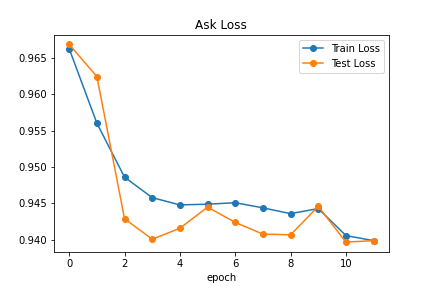
\includegraphics[scale = 0.5]{figs/Ask_Loss.png}
    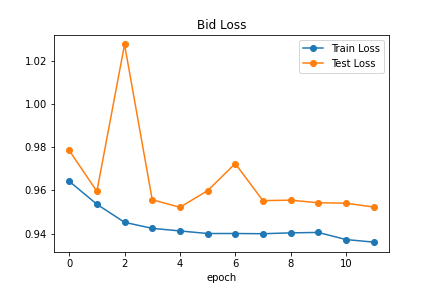
\includegraphics[scale = 0.5]{figs/Bid_Loss.png}
    \caption{\small Training Curve: LEFT: the training history for bid arrivals. RIGHT: the training history for ask arrivals. We see we may continue to train but the result seems to stabilize here. }
    \label{sec2:fig:Loss}
\end{figure}

\begin{figure}
    \centering
    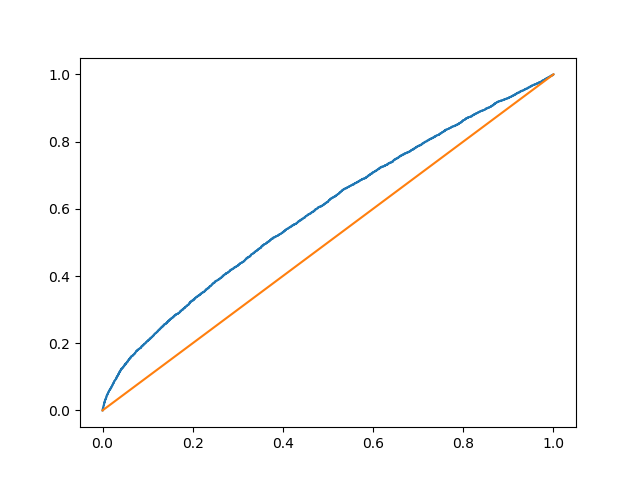
\includegraphics[scale=0.4]{figs/bid_roc.png}
    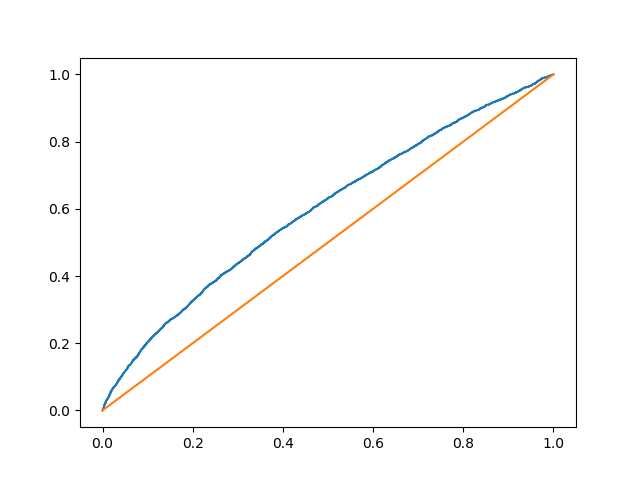
\includegraphics[scale=0.4]{figs/ask_roc.png}
    \caption{\small ROC curve: LEFT: the result for bid arrivals. RIGHT: the result for ask arrivals.}
    \label{sec2:fig:ROC}
\end{figure}

The ROC curve is the curve plotted by adjusting the threshold of the classification. For example, we normally use $0.5$ as the threshold and if probability we predicted is less than 0.5, the label we predict will be 0 and otherwise it will be one. So in the ROC curve, the horizontal axis is the false positive rate axis and the y axis is the true positive rate. For each threshold, we could count the true positive rate and the false positive rate. For a purely guessing model, or for observations that we do not have any a priori information, the ROC curve should be a straight line of $y=x$. This is because, for each sample with hidden label $0$ and that with the hidden label $1$, we have the same probability of labeling them to $1$. Thus, the true positive rate and the false positive rate should be the same. Thus, the ROC curve that is more different from the straight line, the better the model is. 


With the information about ROC cuve, from Fig.\ref{sec2:fig:ROC}, we see the ROC curve is slightly higher than the straight line and this means our model is better than pure guess but it is only slightly better. We may question whether we should continue to train. However, from the training curve, it is shown, the training loss and the test loss both start to converge and stabilize and as a result, we will accept that the deep net already dig out as much information as it can by just utilizing the self correlation. (However, remember we just used a finite window size, we may use an infinite window size and the result may be better but we need more layers for that task)


\section{Data Visualization and Feature Engineering}

Now, if we stick with our original plan, we should continue to train some small models for the data. However, because small parametric models made strong assumptions about the data and they can only discover simple relations between the input and the output, we should expand the features given in the data so that the prediction dependence on the original features will be more sophisticated (although the more complicated dependence is added by hand of us).  In order to put meaningful and helpful features into the model, we should first identify import features and combing those important features to expand the data.

The details of the data visualization is shown in the adjoint \texttt{jupyter-notebook}. For simplicity, here we show some key results that we found in the data visualization. In order to visualize the important features and try to construct new features from them, we first use a correlation matrix to see how the number of order arrivals correlate with each features. We select a bunch of them and the full list of them is in the adjoint \texttt{notebook}. We then make plots to visualize the data. The way we show the data is by plotting the ask and bid order arrivals with each interesting features. In order to have a feeling of the trend, we make bins on the axis and plot the mean or median of the quantities for each bin. 

First, in Fig. \ref{sec3:fig:volume_density}, we plotted the ask and bid order arrivals versus the volume feature. We can see the number and the probability of arrivals of orders decrease with the volume. We interpret this behaviour by the correlation between volume and time. The more volume there is means, there is less time to the close of market and thus, less people will put orders. Since putting order risks exposing traders' intentions to the public and if there is less time for the order to actually transact, the risk is higher than the gain and thus, less people will put order at a later time than at an earlier time. Also, from the histogram of the counts of data, we see there are less data recorded in the small volume portion which means people's trading frequency is high in small volume and is low when the volume is high. This shows people tend to apply their strategies earlier in a day.

\begin{figure}
    \hspace*{-0.6in}
    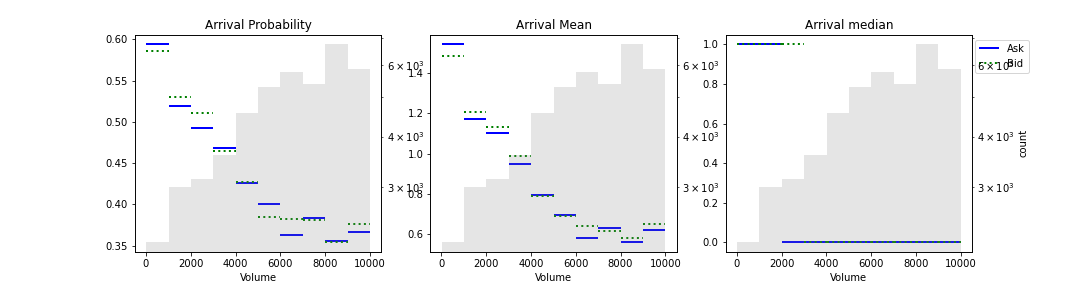
\includegraphics[scale = 0.5]{figs/densities/density_Volume.png}
    \caption{\small Ask and Bid arrivals versus volume. The y axis in the left plot is the probability of order arrivals. The y axis in the middle plot is the mean of order arrivals and the y axis in the right is the median of the order arrivals. The gray bars are the number of observations in each bin. }
    \label{sec3:fig:volume_density}
\end{figure}

\begin{figure}[H]
    \hspace*{-0.6in}
    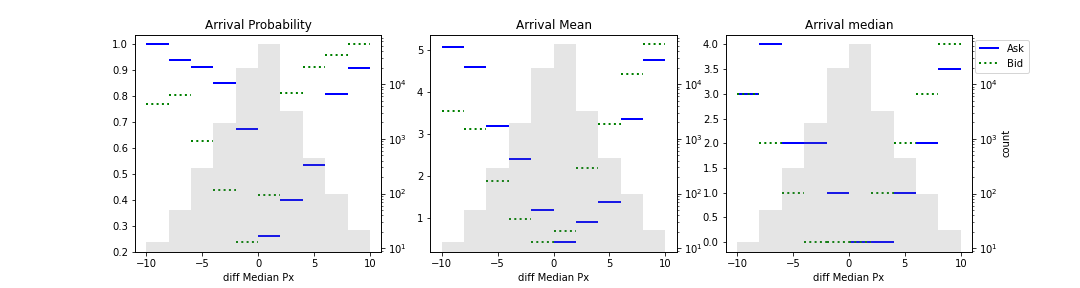
\includegraphics[scale = 0.5]{figs/densities/density_diff Median Px.png}
    \caption{\small Ask and Bid arrivals versus rate change of median price. The y axis in the left plot is the probability of order arrivals.  }
    \label{sec3:fig:diff_median_px_density}
\end{figure}

Another interesting feature is that when we consider the effects of the changing rate of the median price. Here, the median price the middle price of the lowest selling price $a(t)$ and the highest bidding price $b(t)$. From the Fig. \ref{sec3:fig:diff_median_px_density} we see that no matter whether the median price is rising or decreasing, the probability and amount of order arrivals always increase. Specifically, when the median price is increasing, both the bidding orders and the asking orders will increase. However, we believe the asking orders increase as a response of the bidding orders. This is because the asking orders amount increase less severely than the bidding orders. This could interpreted that when the median price are increasing, the value of the stock increases and thus more people want to buy it. As more and more orders bidding with high price, there will be some traders who are satisfied with their profit and are willing to sell their stock. Also, it could be that the selling traders are putting orders with high selling price to try their luck to see whether they will sell it. This happens symmetrically for asking orders. That is when the median price are decreasing, people tend to believe the price of the stock will decrease and thus more people will tend to put ask orders. As a result, some traders will post more bidding orders with low prices to see whether there will be anybody who wants to sell their stock at a relatively low price. 



The last take away we want to mention is the behaviour of the ask and bid orders relative to the highest bidding price and the lowest asking price. We will discuss on Fig.\ref{sec3:fig:bid_ask_price}. The plot shows the increase of bid price directly make the probability of bidding to be one and the bidding quantity increase dramatically. This is may imply that people tend to believe that when people wants to pay more for the stock, the stock will definitely worth more and thus people will bid for it. In the mean time, some trader will post their "phishing" ask orders to see whether there will be people wish to buy with a higher price. In this case, we did not have symmetry for increase and decrease of bidding price. This is because, the bidding price decrease is interpreted as a fluctuation since we are marginalizing the lowest selling price. Thus, if we fix the selling price and just the buying price decreases, this means the demand for the stock is invariant but just some highest price bidding orders are conducted.  In contrast, if the bidding price increases, it must be some people want to buy it but no body can offer it immediately. This must increase the willing to buy in the market. We have exactly symmetric behaviour for asking orders when the ask price decreases. Also from the plots, the green lines in the above plots are just "replaced" by the blue lines but in a mirror symmetric sense. 

\begin{figure}[H]
    \hspace*{-0.6in}
    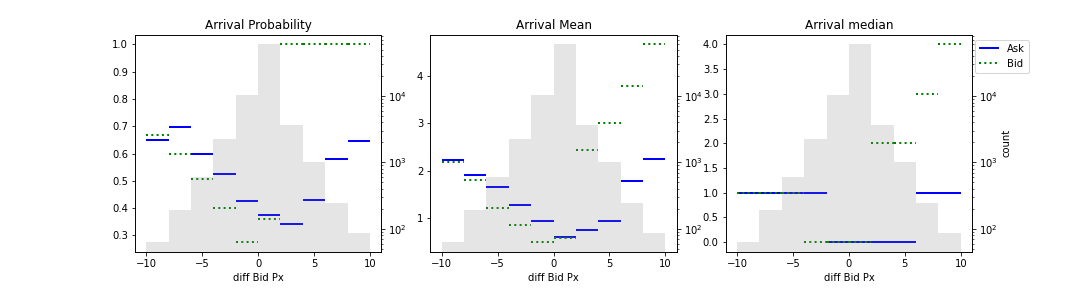
\includegraphics[scale = 0.5]{figs/densities/density_diff Bid Px.png}
    
    \hspace*{-0.6in}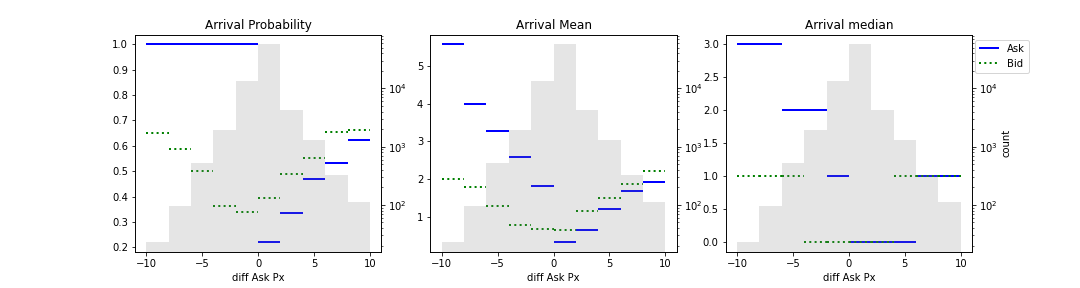
\includegraphics[scale = 0.5]{figs/densities/density_diff Ask Px.png}
    \caption{\small Ask and Bid arrivals versus rate change of Bid Price (upper plots) and Ask Price (lower plots). The y axis in the left plot is the probability of order arrivals. The y axis in the middle plot is the mean of order arrivals and the y axis in the right is the median of the order arrivals. The gray bars are the number of observations in each bin. }
    \label{sec3:fig:bid_ask_price}
\end{figure}

In the last we will summarize what we find are most import in determining the behaviour of the order flows:
\begin{itemize}
    \item \textbf{Bid Taken} (The amount of conducted bid orders between the last time slot and now)
    \item \textbf{Ask Taken} (The amount of conducted bid orders between the last time slot and now)
    \item \textbf{Median Price change rate}
    \item \textbf{Bid Price change rate} (Bid price change relative last time)
    \item \textbf{Ask Price change rate} (Ask price change relative last time)
    \item \textbf{log mean return} (log of relative change of median price $\log(m(t)/m(t-1))$)
    \item \textbf{The price gap} 
\end{itemize}
Although, we filtered out some moderate features that have some effects on the order arrivals, we will keep some of them and let a Lasso regression to determine the important features. Besides, we see some features that have a $V$ shaped effects on the order arrivals. Then, we would add absolute value of those features into the model. This is because, we will focus on using linear models for parametric models. In order for the linear models to capture the V-shaped behaviour, we would use features of $|x|$ for the feature $x$. This is because for a model 
\begin{equation}
    y = ax + b|x|
\end{equation}
the effective slope for $x>0$ would be $a+b$ and the effective slope for $x<0$ would be $a-b$. Thus, linear model will effectively capture the V-shaped behaviour if we added the absolute value. 

\section{Models for Classification}
In this section, we will describe how we constructed models to do classification problem on the order arrivals. We first explained how we select the features and then we will show the structure of our models and the result. 
\subsection{Feature selection and PCA}
In the Data Visualization section, we identified the most important features in determining the arrivals of orders but they are the most important ones and we may not neglect other moderate features a priori. Thus, we utilize an L1 regularization for the logistic model to determine the most import features for the classification. 

In order to make sure our model considers enough information, we added features that we designed from the visualization in the last section. Besides, we also append those features from $1$, $2$ and $5$ steps ago from the current time step. This ensures the model would consider correlations from last few steps. The way we chose the steps is inspired by the Kaggle Competition on Bit Coin price prediction. With all these operation, our data has expanded to $143$ features for each observation and this would be simply too much. Thus, we used our Lasso-Logistic regression, where we implemented the cross validation which selects the best penalty coefficient $\lambda$ for L1 penalty. Finally, we obtained the selected features. However, we find the number of features selected for bid order arrivals are around 40 but the features selected for ask order arrivals is around 80. We found the union of them has around 90 features. In order for our model to consider enough information, we took the union which means we put 90 features into the model. Then, we implemented a PCA to choose the best number of features for our final models. 
\begin{figure}[H]
    \centering
    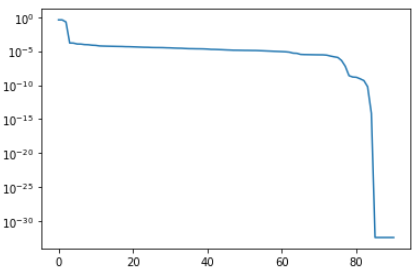
\includegraphics[scale = 0.6]{figs/PCA.png}
    \caption{Principal component analysis for the features selected by either Bid or Ask lasso-logistic regression }
    \label{sec4:fig:PCA}
\end{figure}
It is clear from Fig.\ref{sec4:fig:PCA}, there is no variation for principal components after 80 components. Thus, we would use 80 features as our predictive features to do the classification problem. The exact list of variables that we selected and the features that we did PCA on is explicitly shown in the accompanying notebook. In the next two subsections we will list our models for the classification. 

\subsection{Models for Bid Arrival}
Till now, we used Lasso regression to select the variables and we used PCA to get 80 principal components. Then we will fit our model in predicting the classification. We initialized a bunch of models and we did a preliminary fit for each of the models and try to eliminate some of them by their \texttt{f1} score in the cross validation. After neglecting worst models, we will tune the hyper-parameters in each model. At last, we will fit a stacking model where the first layer of stack is the best model selected with the best hyper-parameters and the second layer will take the input from the first layer as well as the input data to predict a final score. We will show the detail in this second

\begin{table}[H]
    \centering
    \begin{tabular}{c |l| l| l| l }
    \hline \hline 
         model & parameter 1 & parameter 2 & mean f1 score & select   \\ \hline 
         KNN          & Neighbors: 10  &          & 0.4559           & No  \\ \hline 
         SVM          & Reg par: 0.1   &          & 0.7075           &\color{red}{Yes}  \\ \hline 
         QDA          & Reg par: 0.01  &          & 0.6943           &\color{red}{Yes}   \\ \hline  
         Logistic     & Reg par: 0.1   &          & 0.7109           &\color{red}{Yes}   \\ \hline 
         Decision Tree& Depth: 15      &          & 0.6001           & No  \\ \hline 
         AdaBoost     & estimators: 100& depth: 2 & 0.6904           &\color{red}{Yes}   \\ \hline 
         XgBoost      & estimators: 150&          & 0.7007           &\color{red}{Yes}   \\ \hline 
         Extrad Tree  & estimators: 50 &          & 0.6022           & No  \\ \hline 
         Random Forest& estimators: 150& depth: 12& 0.6456           & No  \\ \hline 
         Naive Bayes  &                &          & 0.3686           & No  \\ \hline 
         Gradient Boost&               &          & 0.6663           &\color{red}{Yes}   \\ \hline \hline
    \end{tabular}
    \caption{Models selection for Bid Arrival classification}
    \label{sec4:tab:model_select}
\end{table}

In Table. \ref{sec4:tab:model_select}, we showed the models that we used and the hyper parameters we chose as well as the mean f1 score achieved in the 5 folded cross validation. Here, we see the KNN model performed bad and this is due to the fact that the dimension of features is $80$ and the curse of dimensionality makes the data "sparse" in the high dimensional space and thus, the nearest estimation does not perform well. Besides, the naive Bayes model also did not perform well and this may be because the "independence" assumption is violated in this data set. From the table, we finally choose $6$ models with three of them are boosted or ensemble models with the base model of decision tree. 

We finally stacked the 6 selected models to make the final prediction. The classical stack procedure is that, we divide the data into 5 folds and for each model we trained on $4$ folds and predict on the left over $1$ fold and iterate through the folds. Then, for each model, we collect all the prediction on the left over validation set as a column. Thus, finally, we get a matrix of $6$ columns with each column storing the prediction from each respective model.  Then we feed in the $6$ columns matrix into a final mega-model. However, in this task, we will do it differently. We will append the result from the $6$ models to the PCA transformed input. We would also append the result from the deep net. Finally, we feed this data into the final mega-model which is a logistic regression in our case. 


In figure \ref{sec4:fig:ROC_bid} , we showed the ROC curve on both training and testing data produced by the stacking mode. We see the ROC curve is a great improvement to that produced from the Deep Net. However, we see the ROC curve in the training data set is better and that in the test data set. This could indicate that our stacking model is over-trained on the training data. The final train accuracy reaches around $83.8\%$ but the test accuracy is only $81.7\%$. The result is summarized in table \ref{sec4:tab:bid_result}.

\begin{table}[H]
    \centering
    \caption{Bid arrival classification result}
    \begin{tabular}{c c c}
       \hline \hline 
                 & train      & test     \\ \hline
        f1 score & $0.7505$   & \color{red}{$0.6990$}  \\ 
        accuracy & $83.80\%$  & \color{red}{$81.78\%$} \\ \hline \hline 
    \end{tabular}
    \label{sec4:tab:bid_result}
\end{table}

\begin{figure}
    \centering
    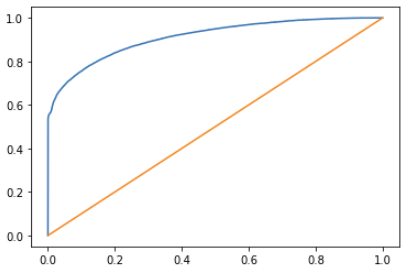
\includegraphics[scale=0.45]{figs/ROC_bid_train.png}
    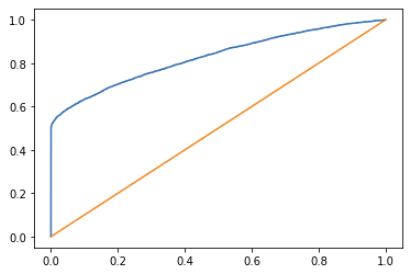
\includegraphics[scale=0.45]{figs/ROC_bid_test.png}
    \caption{\small ROC curve: LEFT: the result for bid arrivals on train data set. RIGHT: the result for bid arrivals on test data set.}
    \label{sec4:fig:ROC_bid}
\end{figure}

\subsection{Models for Ask Arrival}
We did almost the same as in the bid arrival classification for the ask arrival classification. The only difference is that we used different hyper parameters in the model for the final stacking model. Also, in principal, the ask arrival prediction could be different from that of the bid arrivals. Thus, we start from the model selection and re-adjust the hyper parameters. In table, we see similar behaviour for KNN. In principal, we could directly reject KNN since the dimension of features is too large compared to the number of observations. However, it may occur that the decision tree and the random forest to perfomr well in this predcition. Thus, we still include them. The result of the model selection for ask arrivals is shown in table \ref{sec4:tab:ask_model_select}.  We see, the decision tree and random forest still do not perform well. Therefore, we will not re adjust the hyper parameter for those models. Besides, we also find that the Naive Bayes also did not well in this prediction. Basically, we finally chose the same models as in the bid arrival prediction.  

\begin{table}
    \centering
    \begin{tabular}{c |l| l| l| l }
    \hline \hline 
         model & parameter 1 & parameter 2 & mean f1 score & select   \\ \hline 
         KNN          & Neighbors: 10  &          & 0.4559           & No  \\ \hline 
         SVM          & Reg par: 0.1   &          & 0.7075           &\color{red}{Yes}  \\ \hline 
         QDA          & Reg par: 0.001 &          & 0.6920           &\color{red}{Yes}   \\ \hline  
         Logistic     & Reg par: 1.0   &          & 0.7126           &\color{red}{Yes}   \\ \hline 
         Decision Tree& Depth: 6       &          & 0.5314           & No  \\ \hline 
         AdaBoost     & estimators: 100& depth: 2 & 0.6904           &\color{red}{Yes}   \\ \hline 
         XgBoost      & estimators: 150&          & 0.7007           &\color{red}{Yes}   \\ \hline 
         Extra  Tree  & estimators: 50 &          & 0.6022           & No  \\ \hline 
         Random Forest& estimators: 50 & depth: 4 & 0.4019           & No  \\ \hline 
         Naive Bayes  &                &          & 0.3545           & No  \\ \hline 
         Gradient Boost&               &          & 0.6556           &\color{red}{Yes}   \\ \hline \hline
    \end{tabular}
    \caption{Models selection for Bid Arrival classification}
    \label{sec4:tab:ask_model_select}
\end{table}

\begin{table}[H]
    \centering
    \caption{Ask arrival classification result}
    \begin{tabular}{c c c}
       \hline \hline 
                 & train      & test     \\ \hline
        f1 score & $0.7458$   & \color{red}{$0.6843$}  \\ 
        accuracy & $83.93\%$  & \color{red}{$81.47\%$} \\ \hline \hline 
    \end{tabular}
    \label{sec4:tab:ask_result}
\end{table}
    
We did similar procedure as in Bid prediction in the final stacking process. One thing we want to note is that on the second stack of the stacking model, the results from deep nets are appended into the input features. The results from the deep nets are all feeded in without differentiating the bid and ask arrival orders. The final result is also similar to the Bid arrival classification. The ROC curve is plotted in Figure \ref{sec4:fig:ROC_ask}. We see similar behaviour and the stacking model may be over trained on the training data. The final result is shown in Table \ref{sec4:tab:ask_result}. 

In summary, we achieved around $81.5\%$ accuracy in predicting the ask and bid order arrivals. Although the result accuracy is acceptable in some sense but the f1 score is comparably low on the test set. 
\begin{figure}
    \centering
    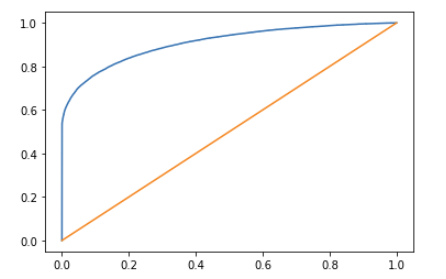
\includegraphics[scale=0.45]{figs/ROC_ask_train.png}
    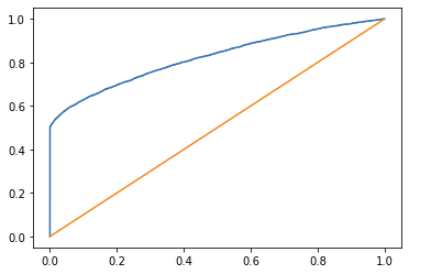
\includegraphics[scale=0.45]{figs/ROC_ask_test.png}
    \caption{\small ROC curve: LEFT: the result for ask arrivals on train data set. RIGHT: the result for ask arrivals on test data set.}
    \label{sec4:fig:ROC_ask}
\end{figure}


\section{Models for Regression}
Since we already made the classification prediction on the ask and bid order arrivals, we could then try to regress on the data to predict the exact amount of order arrivals.  Since we observe that there is only around $3\%$ of orders that is not integer, we round the data set for order arrivals and assume a Poisson distribution for the order arrivals.  The original plan is the same as in the classification where we use different models to predict the mean of the conditional distribution given the data observed before. Then, we try to stack those models. We think this would work since from the data visualization, we see the number of order arrivals is also greatly affected by some specific features such as the bid/ask price.

Since we already know how to classify zero and non-zero order arrivals, we could just regress on the data with positive order arrivals. This means, we would select different data points for bid and ask order predictions since there are data points where only bid order is zero or vice versa. However, when assuming Poisson distribution, we should not neglect zeros. Thus, we subtract $1$ for those observations. Then in the final prediction, we just add one back to get the final result. 

However, after we did a Poisson Regression on the data set, we find the Poisson model only predicts the overall mean of the order arrivals with negligible variations. Thus, our model is not predictive and the variance explained by the Poisson model is only $0.2\%$ which is negligible. This indicates strongly that the features that we use do not contain information in predicting the number of arrivals or at least the linear model we are using cannot extract enough information from them to do the prediction. 

Thus, a good alternative way is to train a \textbf{deep net} with all features from the original data set feeding in so that the deep net could extract correlation for other features and extract dependence of the order arrivals on the other features. In deep net, we do not need to specify an exact model like in linear regression and thus the deep net may extract highly no linear dependence that our linear model fails to. Another alternative is to use \textbf{kernel method} to do the regression. {\color{red}{However, since we do not have enough time, we did not try those two alternatives.}} 

\begin{figure}
    \centering
    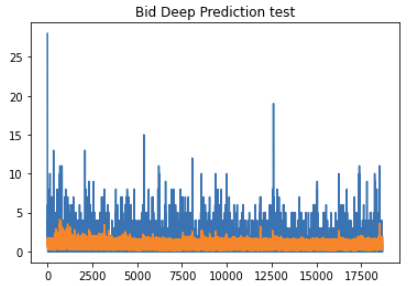
\includegraphics[scale=0.5]{figs/bid_number_pred.png}
    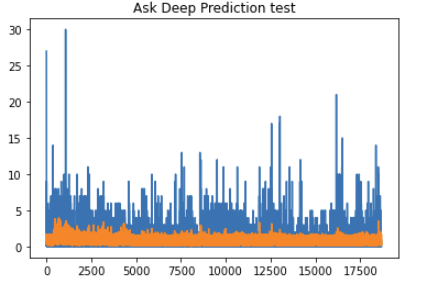
\includegraphics[scale=0.5]{figs/ask_number_pred.png}
    \caption{Order arrival number prediction; LEFT:test data and prediction for  bid order arrivals. RIGHT: test data and prediction for ask order arrivals }
    \label{sec5:fig:number_pred}
\end{figure}

However, our deep net, although only trained on the order arrival data itself, could predict the number of order arrivals. As a result we could use the probability predicted by the classification stacking models and the number of arrivals predicted by the deep net to do the prediction. The final result is shown in the fig.\ref{sec5:fig:number_pred} where the orange line is the prediction while the blue line is the hidden truth for the test data. Here, we see the prediction almost varies with the hidden truth. The quantitative result is shown in table \ref{sec5:tab:regress_result}. 

\begin{table}[H]
    \centering
    \caption{ Order arrival regression result}
    \begin{tabular}{c c c c c }
       \hline \hline 
                    & Bid train      &  Ask train    &  Bid test              & Ask test      \\ \hline
        $R^2$ score & $30.93\%$      &  $30.82\%$    &\color{red}{$32.12\%$}  & \color{red}{$26.69\%$} \\ 
        RMSE        & $1.156 $       &  $1.134$      &\color{red}{$0.955$}    & \color{red}{$1.078$}  \\ \hline \hline 
    \end{tabular}
    \label{sec5:tab:regress_result}
\end{table}




\section{Conclusion}

In combining the Deep Net result with the data and stacking individual models, we achieved acceptable results on the $0$/$1$ classification on the ask and bid order arrivals. However, the regression work to predict the exact number of arrivals is not as good as the classification. This could happen since our deep net only grab a portion of correlation in the history. There may be other correlations in other features such as bid/ask price. We did not consider the long time correlation in those features, although we considered only shift 1, 2, 5 data points. This may not be enough. A good way to improve the regression work is to use deep net on the whole data set. Since in this case, the WaveNet will consider correlation in the features that we neglected in our model. The other way is to use Kernel Non-linear method to do the regression. If time perimting, we could try the two alternative results and see whether there is any improvement. 

\bibliography{reference}
\bibliographystyle{ieeetr}
\end{document}